% Chapter Template

\chapter{Background} % Main chapter title

\label{Chapter2} % Change X to a consecutive number; for referencing this chapter elsewhere, use \ref{ChapterX}

\section{Terminology for Biological Neural Networks}
To understand the concepts at work in this thesis, it is necessary to first familiarize with the biology-inspired terminology that is used to describe the roles and functions of components of the computational models that will be introduced later.\\
First and foremost there are the terms describing the basic components of one neuron communicating with a different neuron as illustrated in Figure \ref{fig:pre_post_neuron}. In principle, such biological neural networks only consist of two types of components, that can have highly variable properties though: synapses which establish data connections, and neurons, which serve as nodes receiving and sending signals over synapses according to a predefined rule set. The neuron on the upstream end of a particular synapse is referred to as the \textit{presynaptic neuron}, while the direct downstream synapse is the \textit{postsynaptic neuron}. Neurons can generally have several in- and outgoing synapses, a synapse on the other hand typically only connects two neurons in a strictly directional manner. Neurons can also be either \textit{excitatory}, meaning that on spiking they can only excite their postsynaptic cells by increasing their membrane potential, or \textit{inhibitory}, meaning that all their spikes inhibit the postsynaptic neuron's membrane potential from rising. This mutual exclusivity of excitation and inhibition is known also as Dale's principle in neuroscience.
\\ \ \\
\begin{figure}[htbp]
    \centering
    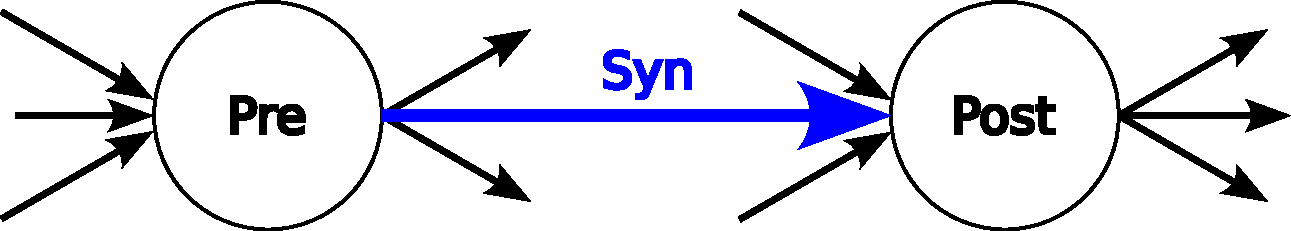
\includegraphics[width=0.9\columnwidth]{Figures/pre_post_neuron.pdf}
    \caption{Basic Synaptic Connection}
    \label{fig:pre_post_neuron}
\end{figure}
If a neuron receives several spikes within a sufficiently small temporal window (dependent on the neuron's characteristics), the potentials triggered by them will be summed together. Depending on whether the incoming spikes triggering these potentials are excitatory or inhibitory, the resulting potentials are called excitatory or inhibitory post-synaptic potentials (EPSP/IPSP). If the membrane potential subsequently reaches a certain threshold (called \textit{action potential}), it will rapidly decrease its membrane potential by unloading it in the form of a spike. Over time the membrane potential deteriorates on itself however, so when the same number of excitatory spikes arrives at the neuron over a longer period of time, or when they are mixed with inhibitory spikes, they might not be able to trigger the action potential. The underlying dynamics of the handling of incoming spikes are referred to as \textit{synaptic integration}, which is why neuron models that are based on this mechanic to determine when to trigger a neuron to fire are called integrate-and-fire (IAF or I\&F) models.\\
The descriptions above are not accurate to the actual proceedings in brain cells and neglect many important biological structural components like dendrites, somata, and axons, to include them in the description of the synapse or neuron. This abstraction is made among other reasons to simplify these models to make them computationally less expensive. 

\section{Synaptic Plasticity}
With the basic structural backgrounds of spiking neural networks out of the way, a synaptic characteristic of critical importance to biological neural networks and the main research object of this thesis is still remaining. The talk is about \textit{synaptic plasticity},  which is generally assumed to be the substrate for learning and memory in cortical circuits \parencite{morrison_diesmann_gerstner_2008}.\\
Plasticity is a property of synapses that makes them form, strengthen, and degrade - for the most part - based on the spiking behavior of the neurons they connect. Due to plasticity being a massively complex mechanic of biological neural networks, that is composed of many different drivers for synaptic weight change, there is no easy way to describe it, which is why over the years, researchers came up with various rules and mathematical models to describe it. In the following two different kinds of plasticity will be briefly introduced.

\subsection{Short-Term Plasticity (STP)} \label{ssec:short_term_plasticity}
As the name already suggests, short-term plasticity operates on rather short timescales in the order of 100s of milliseconds. It can facilitate (STF) or depress (STD) synaptic connections based on the recent spiking history of a presynaptic neuron. A qualitative illustration of STP can be seen in Figure \ref{fig:stp_example} \parencite{morrison_diesmann_gerstner_2008}, where $\text{t}^\text{f}$ denotes an example spike at time $t$ and $x(t)$ is the corresponding postsynaptic membrane potential resulting from the spike.\\
Generally, when a neuron receives a spike, its membrane potential also spikes up and then slowly decreases again as visualized by $x(t)$. Without STP, spikes with very short interspike intervals (ISIs) would continuously increase this way. But based on whether the synapse is depressing or facilitating this behavior is changed. To be more precise, STP in depressing synapses causes the increase in membrane potential to stagnate when many spikes come in with short ISIs by amplifying the decrease after an incoming spike for a short window of time. STP on facilitating synapses on the other hand causes the postsynaptic potential to decrease slower the smaller the ISIs of the incoming spikes are.

\begin{figure}[htbp]
    \centering
    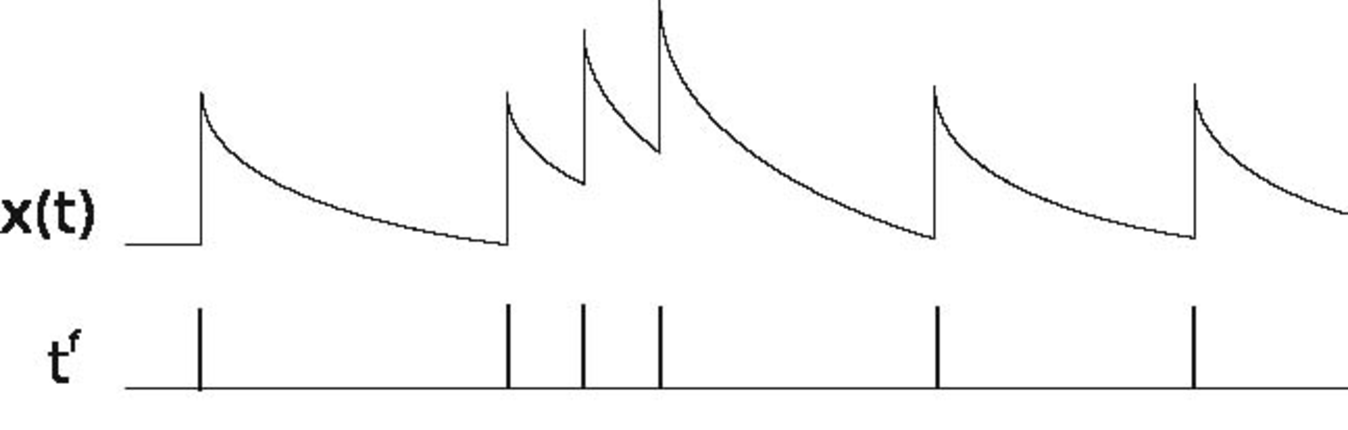
\includegraphics[width=0.9\columnwidth]{Figures/stp_example.pdf}
    \caption{STP Example \parencite{morrison_diesmann_gerstner_2008}}
    \label{fig:stp_example}
\end{figure}


\subsection{Spike-Timing-Dependent Plasticity (STDP)} \label{ssec:spike_timing_dependent_plasticity}
Spike-timing-dependent plasticity is a form of structural plasticity that, unlike STP, allows long-term consolidation of learned behavior by adjusting the efficacy of the synapse based on the learned correlation of firing behavior. This can be better described by Hebb's postulate, an early rule for synaptic plasticity that applies well to STDP:
\begin{displayquote}
\textit{When an axon of cell A is near enough to excite a cell B and repeatedly or persistently takes part in firing it, some growth process or metabolic change takes place in one or both cells such that A’s efficiency, as one of the cells firing B, is increased.}
\end{displayquote}

\begin{wrapfigure}{R}{0.5\textwidth}
    \begin{center}
        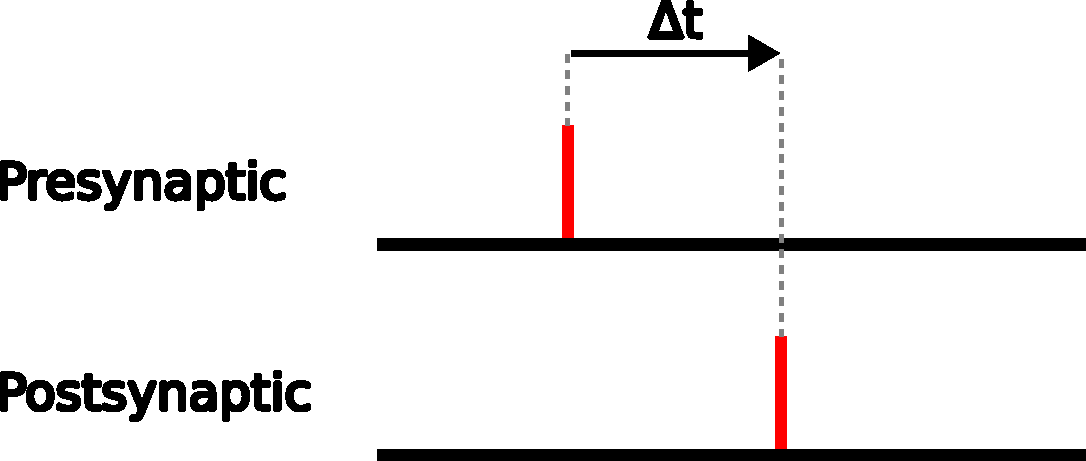
\includegraphics[width=0.48\textwidth]{Figures/pre_post_spikes.pdf}
    \end{center}
\caption{Pre- and Postsynaptic Spikes}
\label{fig:pre_post_spikes}
\end{wrapfigure}
Thus, when a postsynaptic neuron receives a spiking input from a presynaptic source shortly before firing as illustrated in Figure \ref{fig:pre_post_spikes}, the source is more likely to have a causal effect on the postsynaptic neuron, which justifies the facilitation of the connecting synapse. On the other side, if the spiking behavior of the postsynaptic neuron and the source are independent, the connection is degraded. This is a form of correlation-based unsupervised learning, but due to the popularity of Hebb's postulate, it is also referred to as Hebbian learning \parencite{morrison_diesmann_gerstner_2008}.
